%=====================================================================
\section{Embedding-Space Analysis}
\label{sec:analysis}
%=====================================================================

A natural question is why \cinder{} finds concepts that \ember{} misses, and why its directions remove more at moderate edit size.
We expect sharpening to separate the concept from the other rare tokens and make it worth a feature, and \gs{} to set the feature's width from the data.
To test this, we analyze the features themselves, before any edit, on \expnum{38} concepts with 5 factorization seeds each (\ember{}'s 18 and 20 more, 15 of which were added only after the method was frozen), using judge-free measures wherever possible.
Definitions and full results are in \S\ref{app:analyses}.

\paragraph{Sharpening makes the concept pure and valuable}
To see what each step does, we seed a single sparse feature on each concept's lexicon tokens and run it to its fixed point in five matrices: raw, raw with the mean direction $\hat\mu_B$ projected out, centred, whitened only, and sharpened (Figure~\ref{fig:mechanism}b; 38 concepts, 5 seeds).
In the raw matrix the feature drifts toward other rare tokens and ends up only \expnum{24\%} concept-only, although it is among the most valuable features of the fit.
Whitening makes it pure (\expnum{86\%}) but ordinary (\expnum{70th} percentile of feature energies), and sharpening keeps it pure and makes it valuable (\expnum{91st} percentile, higher in \expnum{37 of 38} concepts).
Full fits agree: a lexicon-matching concept feature appears in \expnum{56\%} of raw runs, \expnum{49\%} of whitened-only runs and \expnum{69\%} of sharpened runs (better in \expnum{15} concepts, worse in \expnum{3}), and it carries fewer neutral tokens (\expnum{3.0} vs.\ \expnum{4.5}).
Centring alone, or removing $\hat\mu_B$, does not change how often the concept is found.
Two observations from Harry Potter do not generalize: the raw concept feature usually already ranks near the top by $\rho$ (median \expnum{2}; Harry Potter's 12th place at seed 42 varies from 1st to 48th across seeds), and no selection-free concept direction rises to the top of the spectrum.
Sharpening helps by making a clean cluster worth a feature, not by moving one direction to the top (\S\ref{app:energy}).

\paragraph{The concept's neighbours become related topics}
In the sharpened space, the nearest neighbour of the concept feature is a related topic (magic for Harry Potter, empire for Ancient Rome, computing for Artificial intelligence) at about \expnum{74$^\circ$}, at the \expnum{94th} percentile of an independent word-similarity measure, and the most similar 0.5\% of feature pairs are semantically related (\expnum{75--79th} percentile, against chance for \ember{}; 38 of 38 concepts).
In \ember{}'s matrix the nearest neighbour, at about \expnum{51$^\circ$}, is a feature of unrelated rare tokens, and projecting out the mean direction alone opens the angle to \expnum{74$^\circ$}.
The same direction explains the raw concept feature's large norm, which first drew our attention on Harry Potter (3rd--6th of 100 features): \expnum{97\%} of its excess over a typical feature lies along $\hat\mu_B$.
Orthogonality as such is a property of the metric: each fit is near-orthogonal in its own space, and with $\hat\mu_B$ removed the two dictionaries are equally orthogonal in the embedding space (mean $|\cos|$ \expnum{0.08}).
Concepts rarely split over several features, and when they do the parts are distinct sub-topics, such as Rome and empire for Ancient Rome, which \gs{} keeps apart (\S\ref{app:geometry}).

\paragraph{Widths follow the data}
To test whether a \gs{} width is real, we fix the dictionary, re-solve the coefficients densely, and rank all tokens by their share of the concept feature; the natural tail is where tokens stop being specific to the concept's page (\S\ref{app:gs}).
The natural tail is a property of the direction: doubling the fit's sparsity budget moves it by only \expnum{3} tokens.
On the sharpened matrix, \ember{}'s 1\% cut stops before it for \expnum{25 of 38} concepts, \gs{} widens \expnum{26} of the \expnum{28} features that are cut short, and \gs{} widths follow the tail (Spearman \expnum{0.67} vs.\ \expnum{0.27} for the fixed width; mean error \expnum{30} vs.\ \expnum{42} tokens, $p < 0.001$), robustly across 45 definitions of the tail, though they compress its range and cut the broadest concepts short.
\gs{} changes which tokens a feature keeps, not its direction (cosine \expnum{0.97} with the row-sparse feature, within seed noise), and it helps only after \cs{}: on the raw matrix, the width it adds is mostly neutral tokens and does not track the tail better.
The width varies by about \expnum{4} tokens across seeds when the same feature is found and is unrelated to the feature's index.

\paragraph{The two-way judge recovers concepts lost in the summary}
On 19 concepts, \twj{} accepts a feature that is the concept or a broader version of it in \expnum{82 of 91} runs, against \expnum{61} for \ember{}'s judge, and only \expnum{1 of its 110} acceptances is unrelated.
Most of the added features are broader than the concept (with strict labels, the gain shrinks from \expnum{21} to \expnum{7} runs), and on 15 concepts added after the lexicon prompt was fixed, the lexicon path alone generalizes poorly, while showing the judge each token's source word does generalize (\S\ref{app:twj}).

\paragraph{Abstract concepts stay out of reach}
If concepts are missed because they are quiet, \ember{} should fail most on abstract concepts that lie between louder topics.
On 13 such concepts (e.g., Stoicism, Gnosticism, Gothic architecture) and 4 entity concepts, with blind labels of the top 10 features ($\kappa = \expnum{0.88}$), the top-ranked feature is specific to the concept in \expnum{0 of 65} \ember{} runs and \expnum{0 of 65} \cs{} runs, against \expnum{13} and \expnum{23 of 40} for entity concepts.
For six of the abstract concepts no method places a specific feature in the top 10 in any run; their top features are the parent topics (architecture, religion, painting) and discourse vocabulary.
Sharpening does not recover them (\expnum{$+0.04$} in top-10 presence, n.s.).
We read this as a limit of embedding-level features: an abstract concept is written in a register rather than around a vocabulary of names, and the register is shared with its parent topics.

\paragraph{Sharpening is robust to a blurred contrast}
When up to half of the concept sentences are replaced by sentences from adjacent pages (The Lord of the Rings and Magic for Harry Potter), the sharpened concept feature stays in the top 10 in \expnum{80--93\%} of runs at a mean $\rho$-rank of \expnum{1.8--3.3}, while \ember{}'s mean rank falls from \expnum{4.1} to \expnum{6.9}, as much as with sentences from unrelated pages: the loss is dilution rather than lost contrast.
What adjacency does cause is intrusion: neighbouring tokens (\emph{Tolkien}, \emph{Gandalf}) make up \expnum{14--25\%} of \ember{}'s concept feature and \expnum{5--14\%} of the sharpened one (\S\ref{app:robustness}).

\paragraph{The gain is not circular}
The sharpening target is the concept's own page, which contains the sampled sentences whose tokens we score.
We therefore sharpened toward page sentences outside the sample, toward four other Wikipedia pages about the concept, and, as a control, toward another concept's page (18 concepts, 3 seeds, pre-registered), and scored the features with a strict label (concept-only and either a lexicon word or strongly over-represented on the page relative to Wikipedia).
Both disjoint targets raise the strict purity of the concept feature as much as the page does (\expnum{$+0.06$} vs.\ \expnum{$+0.05$} over \ember{}'s matrix; $p = \expnum{0.003}$ and \expnum{0.009}), keep \expnum{66--75\%} of its gain in concept-vs-neutral separation, and help even on tokens that never occur in the target.
Another concept's page destroys the feature (strict purity \expnum{0.57 $\to$ 0.12}; found in \expnum{2 of 54} runs).
The effect is therefore specific to the concept and does not come from scoring the sharpening text.
Two weaker signals were circular or did not generalize: the coverage measure used to choose $\eta$ improves only with the page target, and the $\rho$-rank of the concept feature does not change on average (the page lifts Harry Potter, Ancient Rome and Halloween but buries Republic of Ireland and Golf under broader co-topics).
On 15 concepts outside the tuning set, every $(\eta, \gamma)$ we tried beats the raw matrix; the default is mid-pack, and $\gamma = 2$ is slightly better (\S\ref{app:cs-circ}).

\paragraph{Features extrapolate only to a few unsampled tokens}
\ember{} edits only tokens of the 300 sampled sentences, and the multilingual pipeline samples 30 per language, so concept tokens that occur only in unsampled sentences are missed unless the fixed dictionary extends to them.
On 17 concepts with about \expnum{730} such tokens each, labelled blindly, roughly one in four extrapolated tokens is concept-specific under every rule we tried (top-10 precision \expnum{0.18--0.27}, against \expnum{0.065} at random), about a third are unrelated, and re-solving the sparse codes recovers only \expnum{4\%} of the concept-specific tokens the sample missed.
On \ember{}'s raw dictionary, projecting onto the concept feature mostly ranks token rarity (Spearman \expnum{0.70} with Wikipedia rarity), so a joint least-squares solve is needed; in the sharpened space the concept feature is nearly orthogonal to the rest of the dictionary (largest $|\cos|$ \expnum{0.28} vs.\ \expnum{0.64}) and the two agree.
The low precision is a property of rare tokens rather than of extrapolation: \expnum{87\%} of unsampled page tokens occur once on the page, and at one occurrence the in-sample support is no more precise.
Extrapolation is therefore a small supplement; for the multilingual pipeline, sampling more sentences is the better lever (\S\ref{app:extrapolation}).

\paragraph{The first layer reads the shared mean, not low-variance directions}
\cinder{}'s edit is read by the model's first layer about as strongly as a random direction, while \ember{}'s and \cinderz{}'s edits are read about twice as strongly (Figure~\ref{fig:read}).
A natural explanation would be that whitening moves the edit into directions of low background variance, which the model ignores.
The data reject it.
The first layer reads low-variance directions \emph{more} strongly than average (\expnum{3.4$\times$} for the lowest 1\% of the eigendirections of $\Sigma_B$), and once the background mean $\mu_B$ is projected out, \ember{}'s and \cinder{}'s edits lie in the same part of the spectrum and are read alike (\expnum{1.31$\times$} vs.\ \expnum{1.32$\times$}, 27 concepts).
The whole gap is the mean term of \S\ref{sec:cinderz}: re-solving \ember{}'s own dictionary on centred embeddings lowers its read strength to \cinder{}'s level (\expnum{1.09$\times$}), and the same holds on Llama, where the mean direction is read at \expnum{20$\times$}.
Whitening thus decides which tokens an edit touches and by how much, not where in the embedding space the edit lies.
The mean term is also most of what aligns an edit with the token it changes (cosine \expnum{0.50} vs.\ \expnum{0.30}, but \expnum{0.31} vs.\ \expnum{0.29} without it), which suggests that part of what makes uncentred edits strong is generic rather than conceptual (\S\ref{app:edit}).

\begin{figure*}[t]
  \centering
  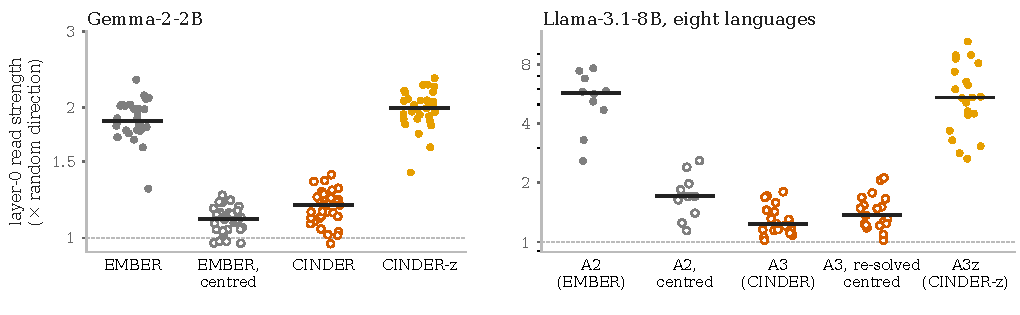
\includegraphics[width=\textwidth]{figures/read_decomposition.pdf}
  \caption{First-layer read strength of each edit, relative to a random direction, per concept (dots) with medians (bars). Re-solving \ember{}'s dictionary on centred embeddings brings its read strength down to \cinder{}'s, and adding the mean term back (\cinderz{}, A3z) raises it again, on Gemma-2-2B (left; concepts with an edit, mean over seeds) and in the multilingual Llama-3.1-8B fits (right). Filled markers: uncentred edits; open markers: centred edits.}
  \label{fig:read}
\end{figure*}
